\chapter{数组}

\section{数组}

\subsection{数组(Array)}

数组是数据结构中最简单的结构,很多编程语言都内置数组。数组是有限个相同类型的变量所组成的集合,数组中的每一个变量被称为元素。 \\

创建数组时会在内存中划分出一块连续的内存,将数据按顺序进行存储,数组中的每一个元素都有着自己的下标(index),下标从0开始一直到数组长度-1。因为数组在存储数据时是按顺序存储的,存储数据的内存也是连续的。 \\

对于数组来说,读取元素是最简单的操作。由于数组在内存中顺序存储,所以只要给出数组的下标,就可以读取到对应位置的元素。像这种根据下标读取元素的方式叫作随机读取。但是需要注意的是,数组的下标范围必须在0到数组长度-1之内,否则会出现数组越界。数组读取元素的时间复杂度是$ O(1) $。 \\

数组拥有非常高效的随机访问能力,只要给出下标,就可以用常量时间找到对应元素。有一种高效查找元素的算法叫作二分查找,就是利用了数组的这个优势。 \\

数组的劣势体现在插入和删除元素方面。由于数组元素连续紧密地存储在内存中,插入、删除元素都会导致大量元素被迫移动,影响效率。总的来说,数组所适合的是读操作多、写操作少的场景。 \\

\mybox{更新数组元素}

\begin{lstlisting}[language=Python]
arr = {3, 1, 2, 5, 4, 9, 7, 2}
arr[5] = 10
print(arr[5])
\end{lstlisting}

\newpage

\section{查找算法}

\subsection{顺序查找(Sequence Search)}

顺序查找也称线性查找,是一种按照序列原有顺序进行遍历比较查询的基本查找算法。 \\

对于任意一个序列以及一个需要查找的元素(关键字),将关键字与序列中元素依次比较,直到找出与给定关键字相同的元素,或者将序列中的元素与其都比较完为止。若某个元素的值与关键字相等,则查找成功;如果直到最后一个元素,元素的值和关键字比较都不等时,则查找不成功。 \\

最好的情况就是在第一个位置就找到,算法时间复杂度为$ O(1) $。 \\

最坏情况是关键字不存在,需要进行$ n $次比较,时间复杂度为$ O(n) $。 \\

平均查找次数为$ (n + 1) / 2 $,平均时间复杂度为$ O(n) $。 \\

\mybox{顺序查找}

\begin{lstlisting}[language=C]
int sequenceSearch(int *arr, int n, int key) {
    for(int i = 0; i < n; i++) {
        if(arr[i] == key) {
            return i;
        }
    }
    return -1;
}
\end{lstlisting}

\subsection{二分查找(Binary Search)}

二分查找法也称折半查找,是一种效率较高的查找方法。折半查找要求线性表必须采用顺序存储结构,而且表中元素按关键字有序排列。 \\

算法思想是假设表中元素是按升序排列,将表中间位置的关键字与查找关键字比较,如果两者相等,则查找成功;否则利用中间位置记录将表分成前、后两个子表,如果中间位置的关键字大于查找关键字,则进一步查找前一子表,否则进一步查找后一子表。重复以上过程,直到找到满足条件的记录,使查找成功,或直到子表不存在为止,此时查找不成功。 \\

二分查找法的时间复杂度为$ O(logn) $。 \\

\mybox{二分查找}

\begin{lstlisting}[language=C]
int binarySearch(int *arr, int n, int key) {
    int start = 0;
    int end = n - 1;
    while(start <= end) {
        int mid = (start + end) / 2;
        if(arr[mid] == key) {
            return mid;
        } else if(arr[mid] < key) {
            start = mid + 1;
        } else {
            end = mid - 1;
        }
    }
    return -1;
}
\end{lstlisting}

\newpage

\section{数组元素插入与删除}

\subsection{插入元素}

在数组中插入元素存在3种情况:

\subsubsection{尾部插入}

直接把插入的元素放在数组尾部的空闲位置即可。

\begin{figure}[H]
    \centering
    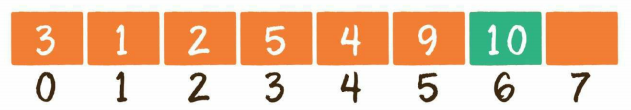
\includegraphics[scale=0.9]{img/C2/2-3/1.png}
\end{figure}

\subsubsection{中间插入}

首先把插入位置及后面的元素向后移动,腾出位置,再把要插入的元素放入该位置上。

\begin{figure}[H]
    \centering
    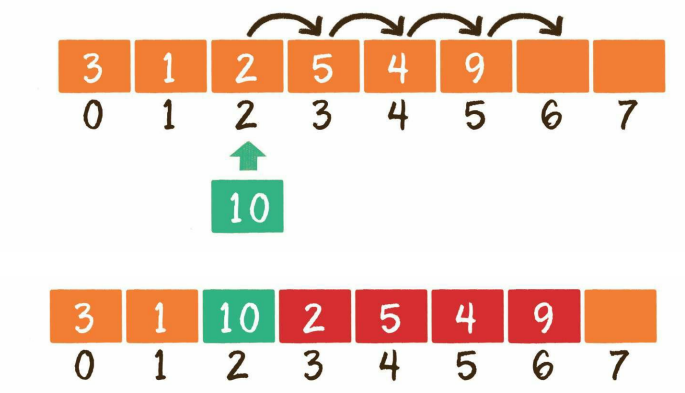
\includegraphics[scale=0.9]{img/C2/2-3/2.png}
\end{figure}

\mybox{插入元素}

\begin{lstlisting}[language=C]
int insert(int *arr, int n, int index, int val) {
    if(index < 0 || index >= n) {
        return n;
    }
    for(int i = n - 1; i >= index; i--) {
        arr[i+1] = arr[i];
    }
    arr[index] = val;
    n++;
    return n;
}
\end{lstlisting}

\subsubsection{超范围插入}

如果数组不断插入新的元素,元素数量超过了数组的最大长度,数组岂不是要撑爆了? \\

数组的长度在创建时就已经确定了,要实现数组的扩容,只能创建一个新数组,长度是旧数组的2倍,再把旧数组中的元素全部复制过去,这样就实现了数组的扩容。 \\

数组插入元素最好情况是尾部插入,无需移动任何元素,时间复杂度为$ O(1) $。最坏情况是在第一个位置插入,这样就需要移动后面所有$ n - 1 $个元素,时间复杂度为$ O(n) $。因此,总体的时间复杂度为$ O(n) $。

\subsection{删除元素}

数组的删除操作与插入操作过程相反,如果被删除的元素位于数组中间,其后的元素都需要向前挪动一位。

\begin{figure}[H]
    \centering
    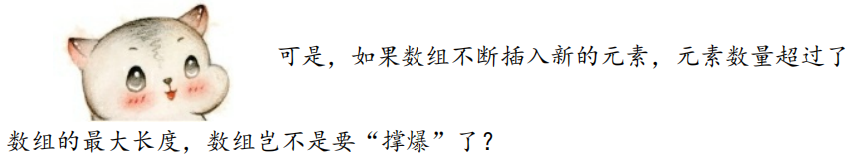
\includegraphics[scale=0.8]{img/C2/2-3/3.png}
\end{figure}

\mybox{删除元素}

\begin{lstlisting}[language=C]
int delete(int *arr, int n, int index) {
    if(index < 0 || index >= n) {
        return n;
    }
    for(int i = index + 1; i < n; i++) {
        arr[i-1] = arr[i];
    }
    n--;
    return n;
}
\end{lstlisting}

数组的删除操作,由于只涉及元素的移动,时间复杂度为$ O(n) $。 \\

对于删除操作,其实还存在一种取巧的方式,前提是数组元素没有顺序要求。如需要删除数组中某个元素,可直接把最后一个元素复制到被删除元素的位置,然后再删除最后一个元素。这样一来,无须进行大量的元素移动,时间复杂度降低为$ O(1) $。当然,这种方式只作参考,并不是删除元素主流的操作方式。

\newpage